\documentclass{article}
\usepackage{graphicx}
\usepackage{hyperref}



\begin{document}

\title{$Z\to e^+e^-$ Data Analysis Tutorial}
\author{Javier Duarte, Cristian Pena, Valere Lambert}
\maketitle

\tableofcontents

\section{Introduction}
You should receive a skeleton \texttt{Zee.C} file and an input \texttt{treeArray.root} file. You will need to re-install root according to the revised directions given here:\\
\url{https://docs.google.com/document/d/1ss5EbpSYidwja7AHelUwNc3VRPqAjJ6cJ3jvDSl1244/edit}

Take some time to aquaint yourself with the code. It initializes a variable \texttt{mee} which represents the invariant mass of an electron and a positron in the collision event. Then it loads data from the \texttt{treeArray.root} file. Finally it plots the data and prints the resulting graph in a \texttt{Zee.pdf} file.

Running the code,
\begin{verbatim}
root -l Zee.C
\end{verbatim}
creates an output \texttt{Zee.pdf} file, shown in Fig.~\ref{fig:Zee}, which illustrates a histogram of the invariant mass spectrum for an electron positron pair in \emph{real} CMS data taken at center-of-mass energy of 8 TeV in 2012.
\begin{figure}
    \centering
    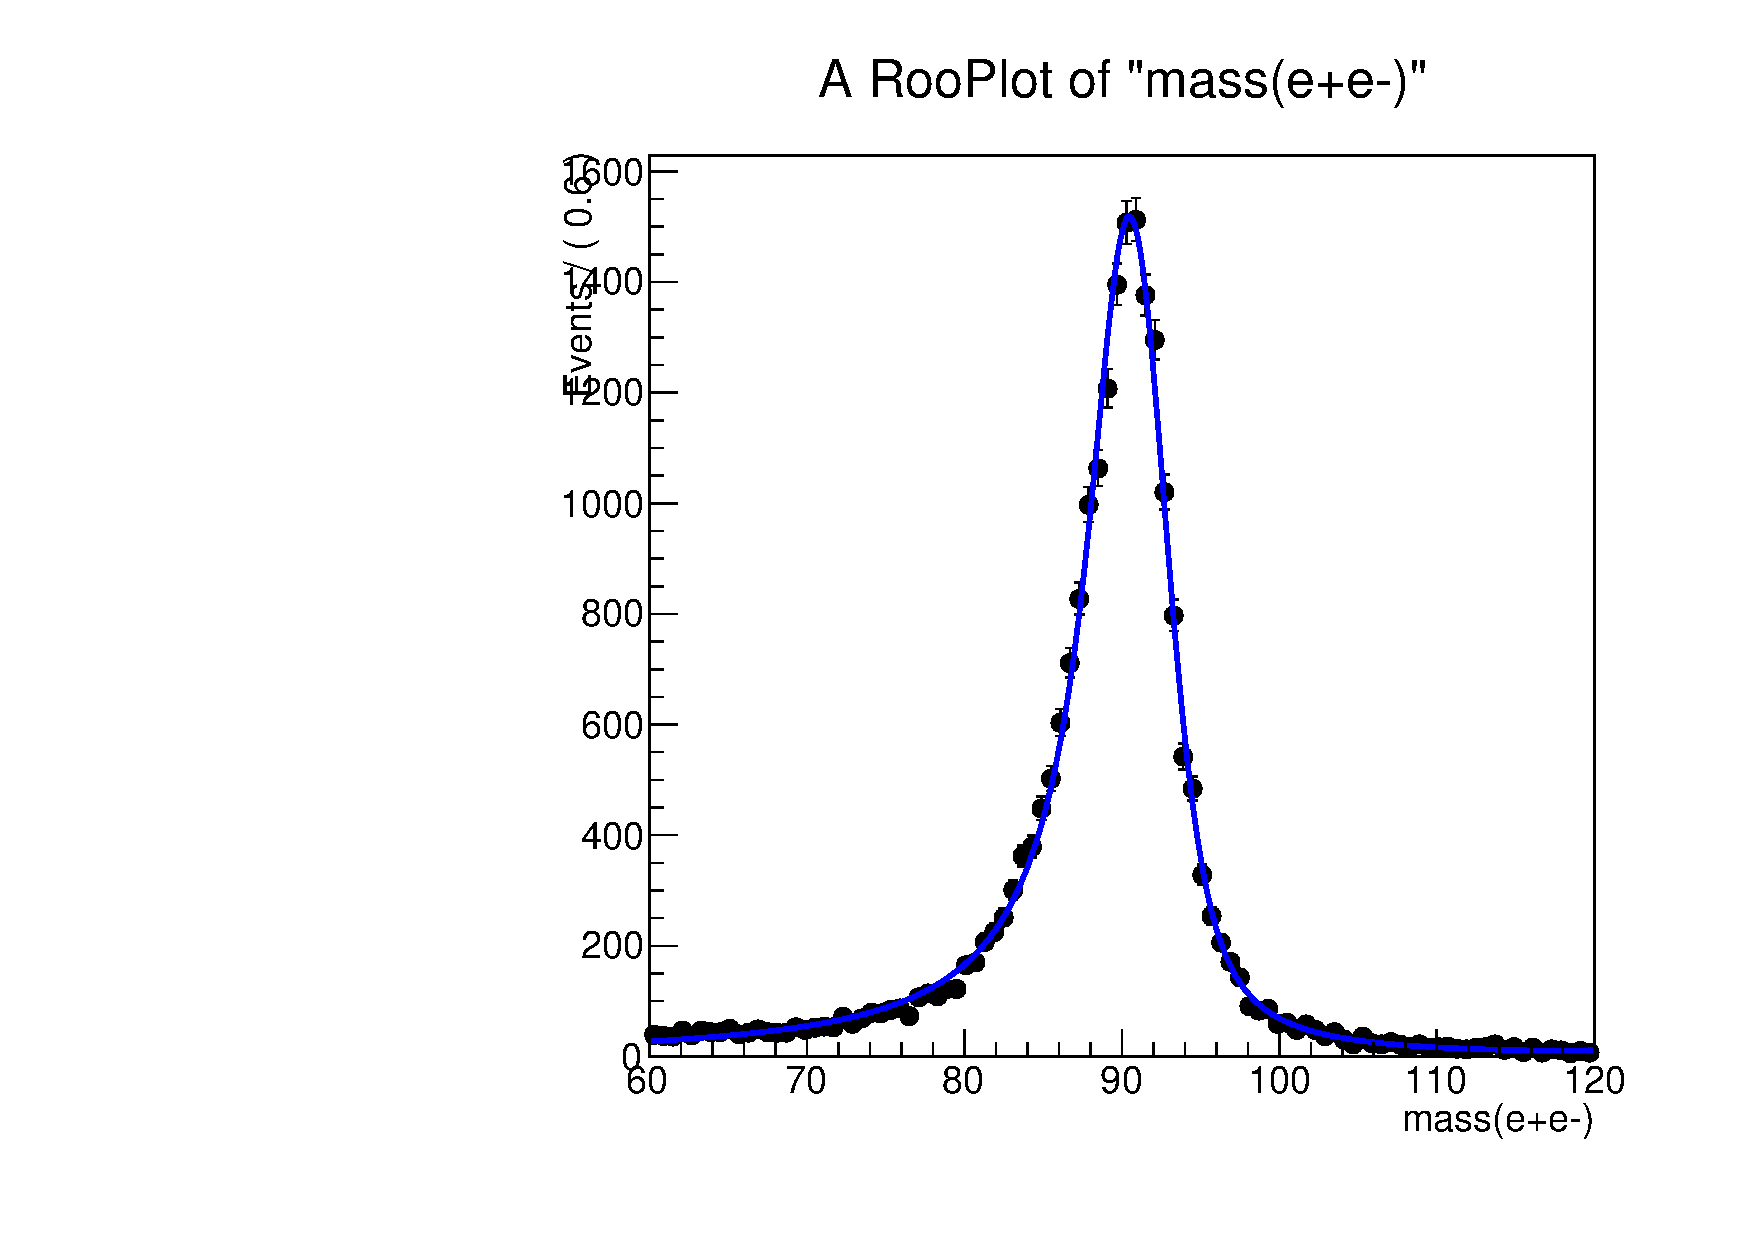
\includegraphics[width=2.0in]{Zee.pdf}
    \caption{Invariant mass spectrum}
    \label{fig:Zee}
\end{figure} 

\section{Maximum Likelihood Fits}
In this section, you will familiarize yourself with the practical
aspects of performing a maximum likelihood fit to data using
\textsc{RooFit} in the \textsc{ROOT} framework.

\subsection{Fit with a Gaussian Distribution}

Now, add the following code to the file
\begin{verbatim}
RooRealVar mean("mean","mean",90,60,120) ;
RooRealVar sigma("sigma","sigma",5,0,20);
RooGaussian gaus("gauss","gaus",mee,mean,sigma);  
\end{verbatim}
after the initialization of the variable \texttt{mee}.

Add the code 
\begin{verbatim}
RooFitResult *fr = gaus.fitTo(*data,Save());
fr->Print("v");  
\end{verbatim}
to perform a fit to the data with a Gaussian distribution and print out the result (in the terminal). Finally, add the code
\begin{verbatim}
gaus.plotOn(frame);
\end{verbatim}
after the line reading \texttt{data->plotOn(frame);} executing the file, 
\begin{verbatim}
root -l Zee.C
\end{verbatim} 
you should now have a modified \texttt{Zee.pdf} that resembles Fig.~\ref{fig:Zee_gaus}.
\begin{figure}
    \centering
    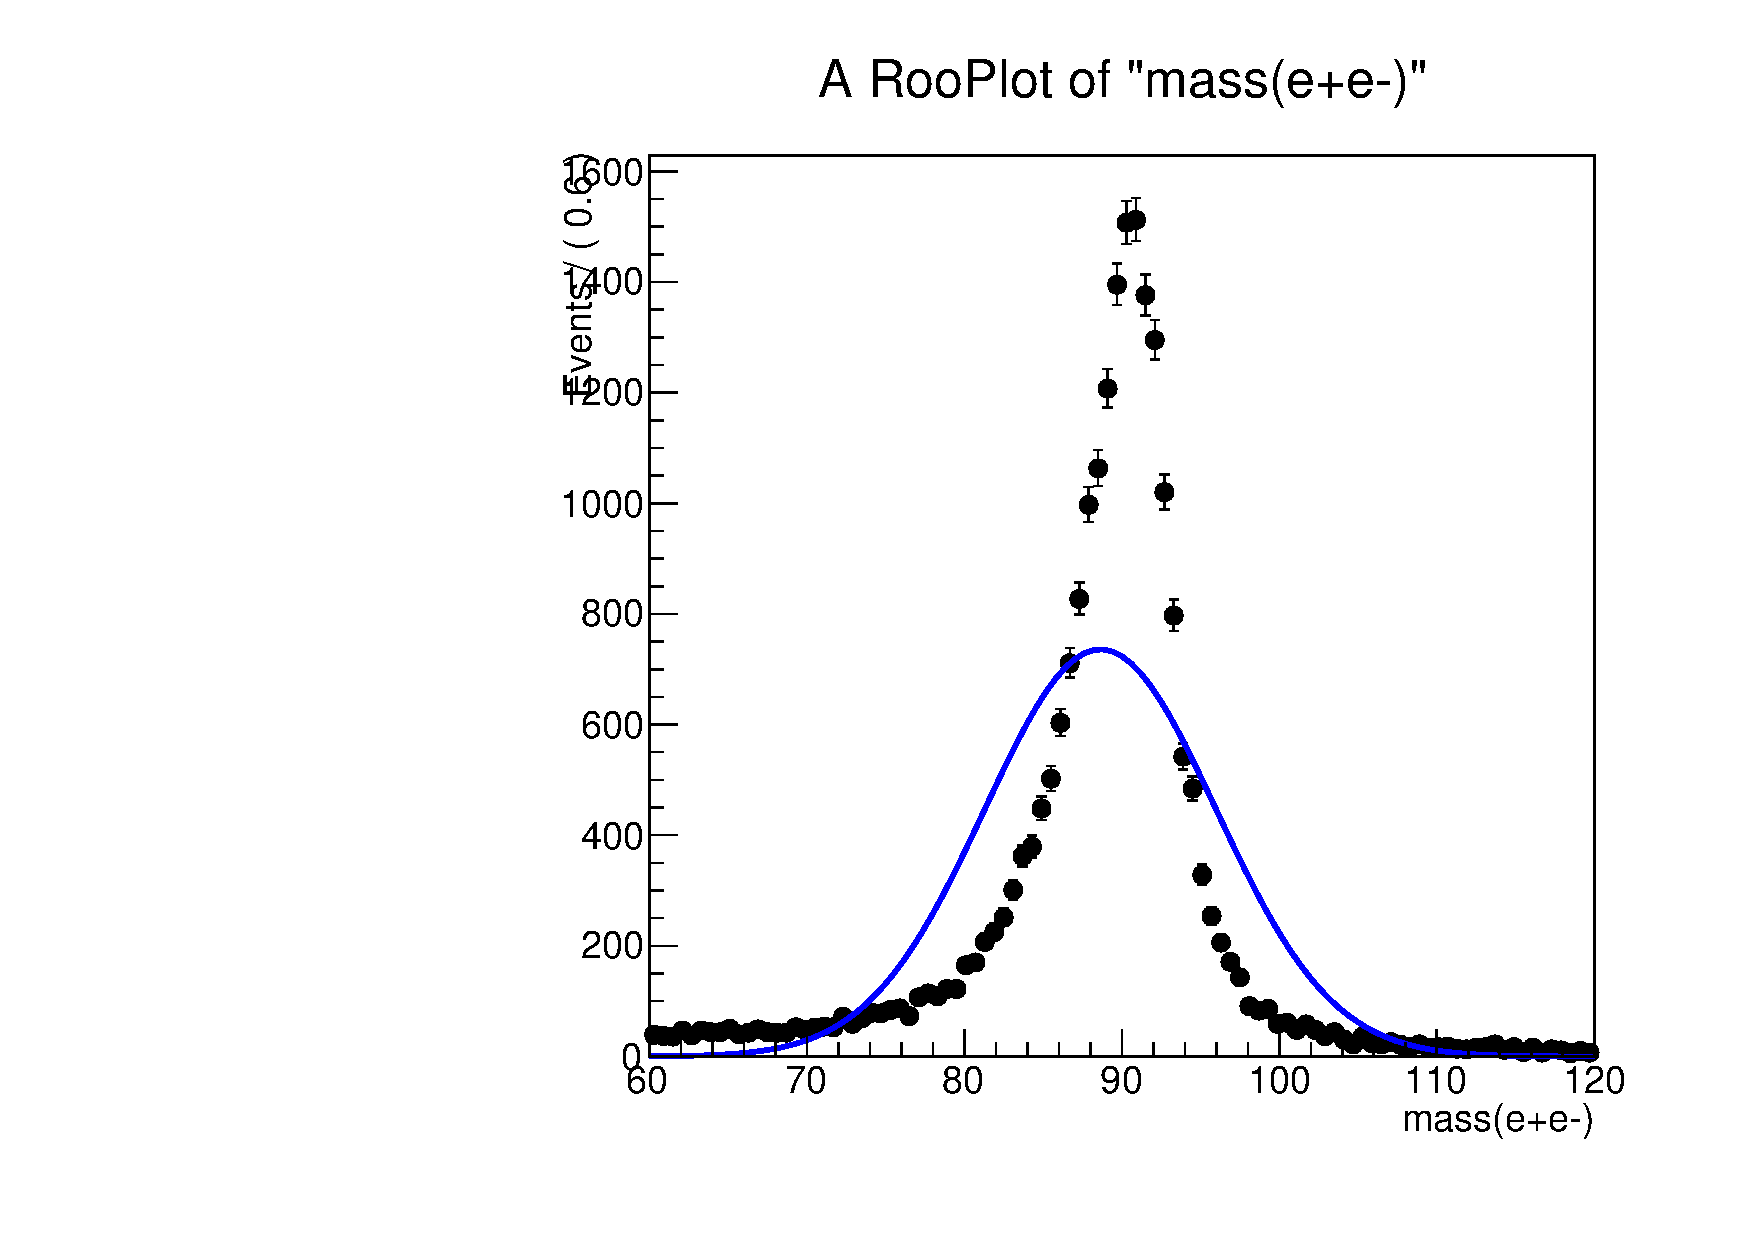
\includegraphics[width=2.0in]{Zee_gauss.pdf}
    \caption{Invariant mass spectrum fit with a Gaussian distribution.}
    \label{fig:Zee_gaus}
\end{figure} 
The Gaussian distribution is often a good first-approximation when fitting
data that has a well defined mode (peak) and spread (width). Its
functional form is parameterized by these two numbers: $\mu$ (mean,
mode, median) and $\sigma$ (standard deviation). Ignoring an overall
normalization constant, 
\begin{equation}
f(x) = e^{-(x-\mu)^2/2\sigma^2}
\end{equation}
Notice, however, that in this case the fit to the data is not very good.

\subsection{Fit with a Relativistic Breit-Wigner Distribution}
Now, instead of adding the code from the previous section (i.e. you should comment out the code from the previous section), add the following code to the file
\begin{verbatim}
RooRealVar bwMean("mZ","BW Mean", 90, 60, 120);
RooRealVar bwWidth("GammaZee", "BW Width", 2, 0, 10);
RooBreitWigner bw("bw", "bw", mee, bwMean, bwWidth);  
\end{verbatim}
after the initialization of the variable \texttt{mee}. 

Add the code 
\begin{verbatim}
RooFitResult *fr = bw.fitTo(*data,Save());
fr->Print("v");  
\end{verbatim}
to perform the fit and print out the result (in the terminal).

Finally, add the code
\begin{verbatim}
bw.plotOn(frame);
\end{verbatim}
after the line reading \texttt{data->plotOn(frame);}. After executing the file, 
\begin{verbatim}
root -l Zee.C
\end{verbatim}
you should now have a modified \texttt{Zee.pdf} that resembles Fig.~\ref{fig:Zee_bw}.
\begin{figure}
    \centering
    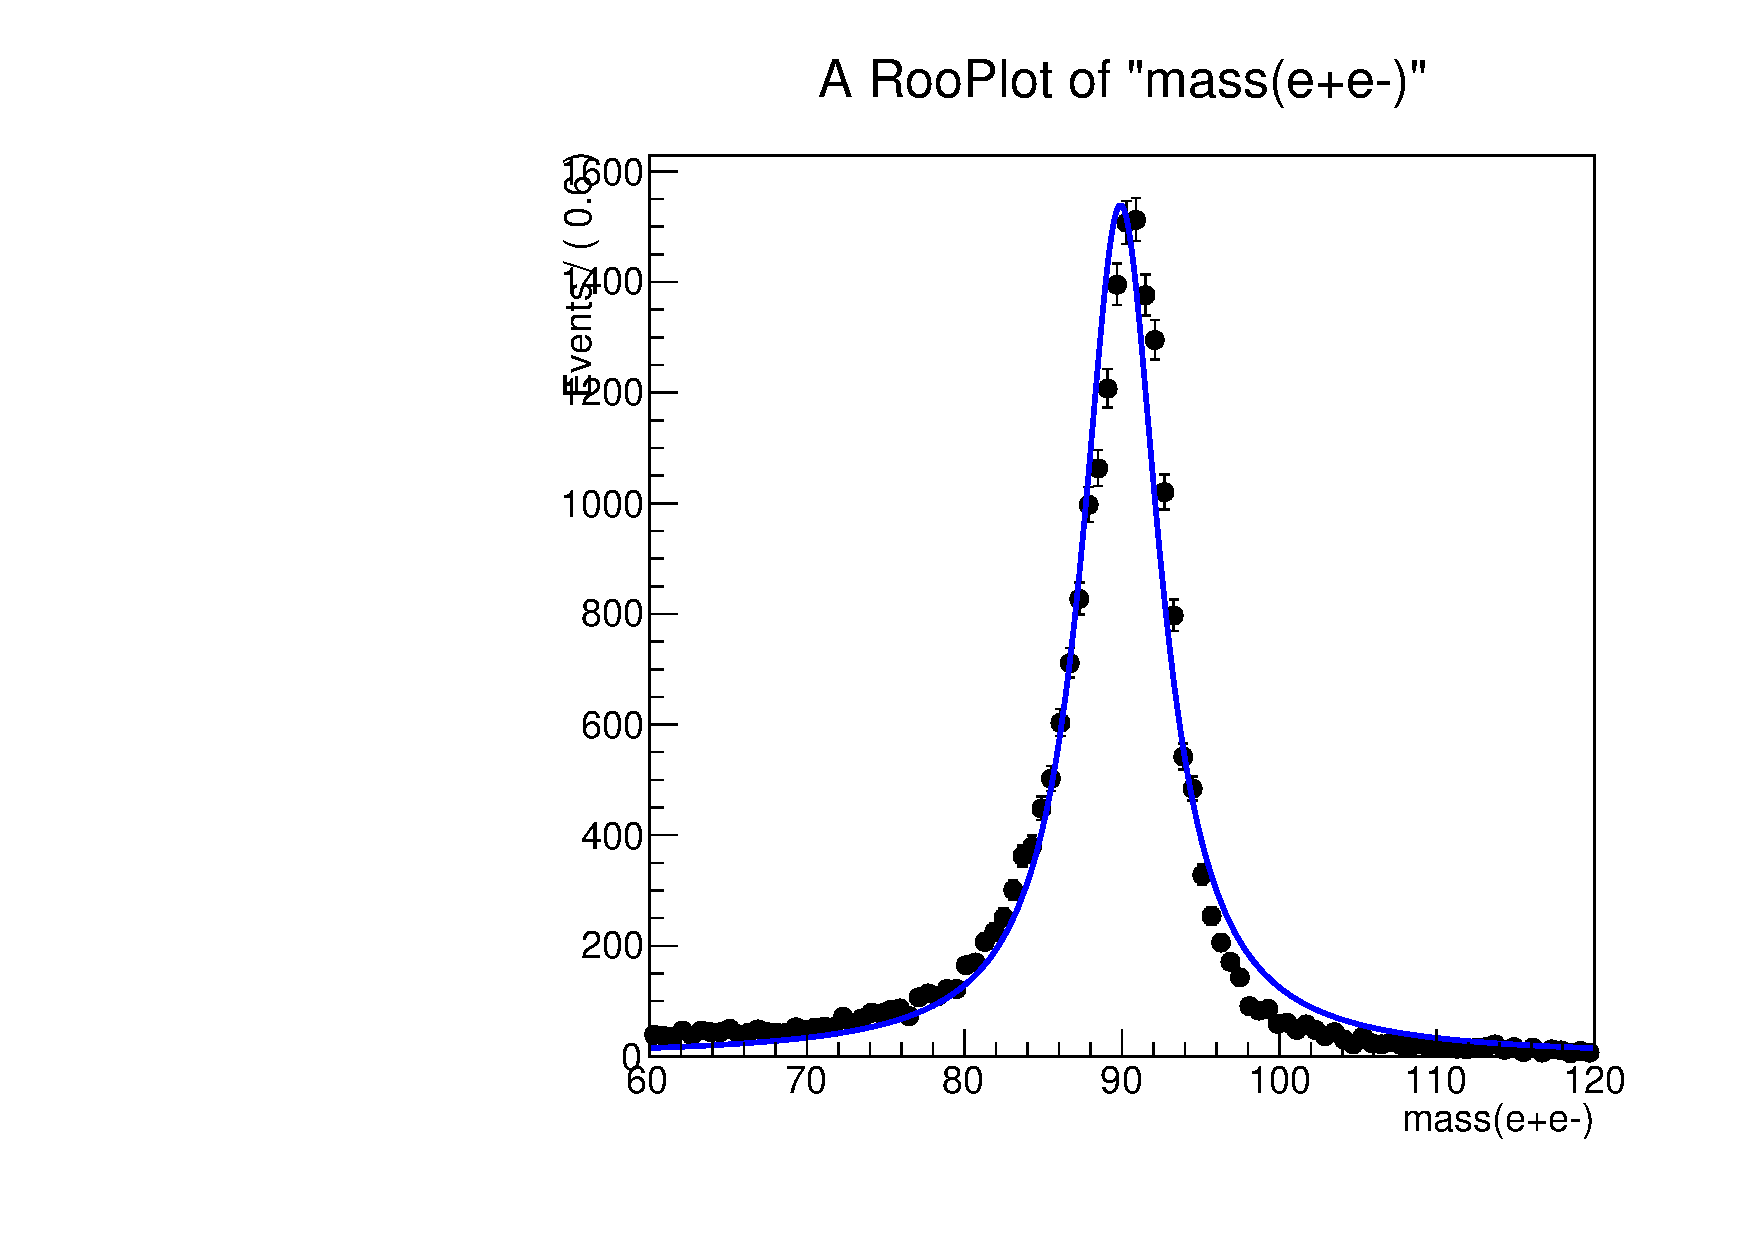
\includegraphics[width=2.0in]{Zee_bw.pdf}
    \caption{Invariant mass spectrum fit with a Relativistic Breit-Wigner distribution.}
    \label{fig:Zee_bw}
\end{figure} 

This code is intended to fit the mass spectrum with a Relativistic
Breit-Wigner distribution, which you can read more about on
\href{http://en.wikipedia.org/wiki/Relativistic_Breit\%E2\%80\%93Wigner_distribution}{Wikipedia}
or in particle physics textbooks. Its functional form is (ignoring an overall normalization constant)
\begin{equation}
f(x) = \frac{1}{(x-\mu)^2+\frac{1}{4}\Gamma^2}
\end{equation}

Notice the fit is much improved with respect to the last iteration.

\subsection{Fit with a Relativistic Breit-Wigner Distribution Convoluted with a Crystal Ball Distribution}
Now add the following code instead of the code from the previous sections.
\begin{verbatim}
RooRealVar cbBias ("cbBias", "CB Bias", -.5, -10, 10);
RooRealVar cbSigma("cbSigma", "CB Width", 5.7, 0.02, 10.0);
RooRealVar cbCut  ("cbCut","CB Cut",1.05, 0.1, 3.0);                              
RooRealVar cbPower("cbPower","CB Order", 2.45, 0.1, 20.0);
RooRealVar bwMean("mZ","BW Mean", 91.1876, 80, 100);
RooRealVar bwWidth("GammaZee", "BW Width", 2.4952, 0, 10);
RooBreitWigner bw("bw", "bw", mee, bwMean, bwWidth);
RooCBShape  cball("cball", "Crystal Ball", mee, cbBias, cbSigma, cbCut, cbPower);
RooFFTConvPdf model("model", "bw X crystal ball", mee, bw, cball);
\end{verbatim}
after the initialization of the variable \texttt{mee}.

Add the code 
\begin{verbatim}
RooFitResult *fr = model.fitTo(*data,Save());
fr->Print("v");  
\end{verbatim}
to perform the fit and print out the result (in the terminal).

Finally, add the code
\begin{verbatim}
model.plotOn(frame);
\end{verbatim}
after the line reading \texttt{data->plotOn(frame);}

You should now have a modified \texttt{Zee.pdf} that resembles Fig.~\ref{fig:Zee_conv}.
\begin{figure}
    \centering
    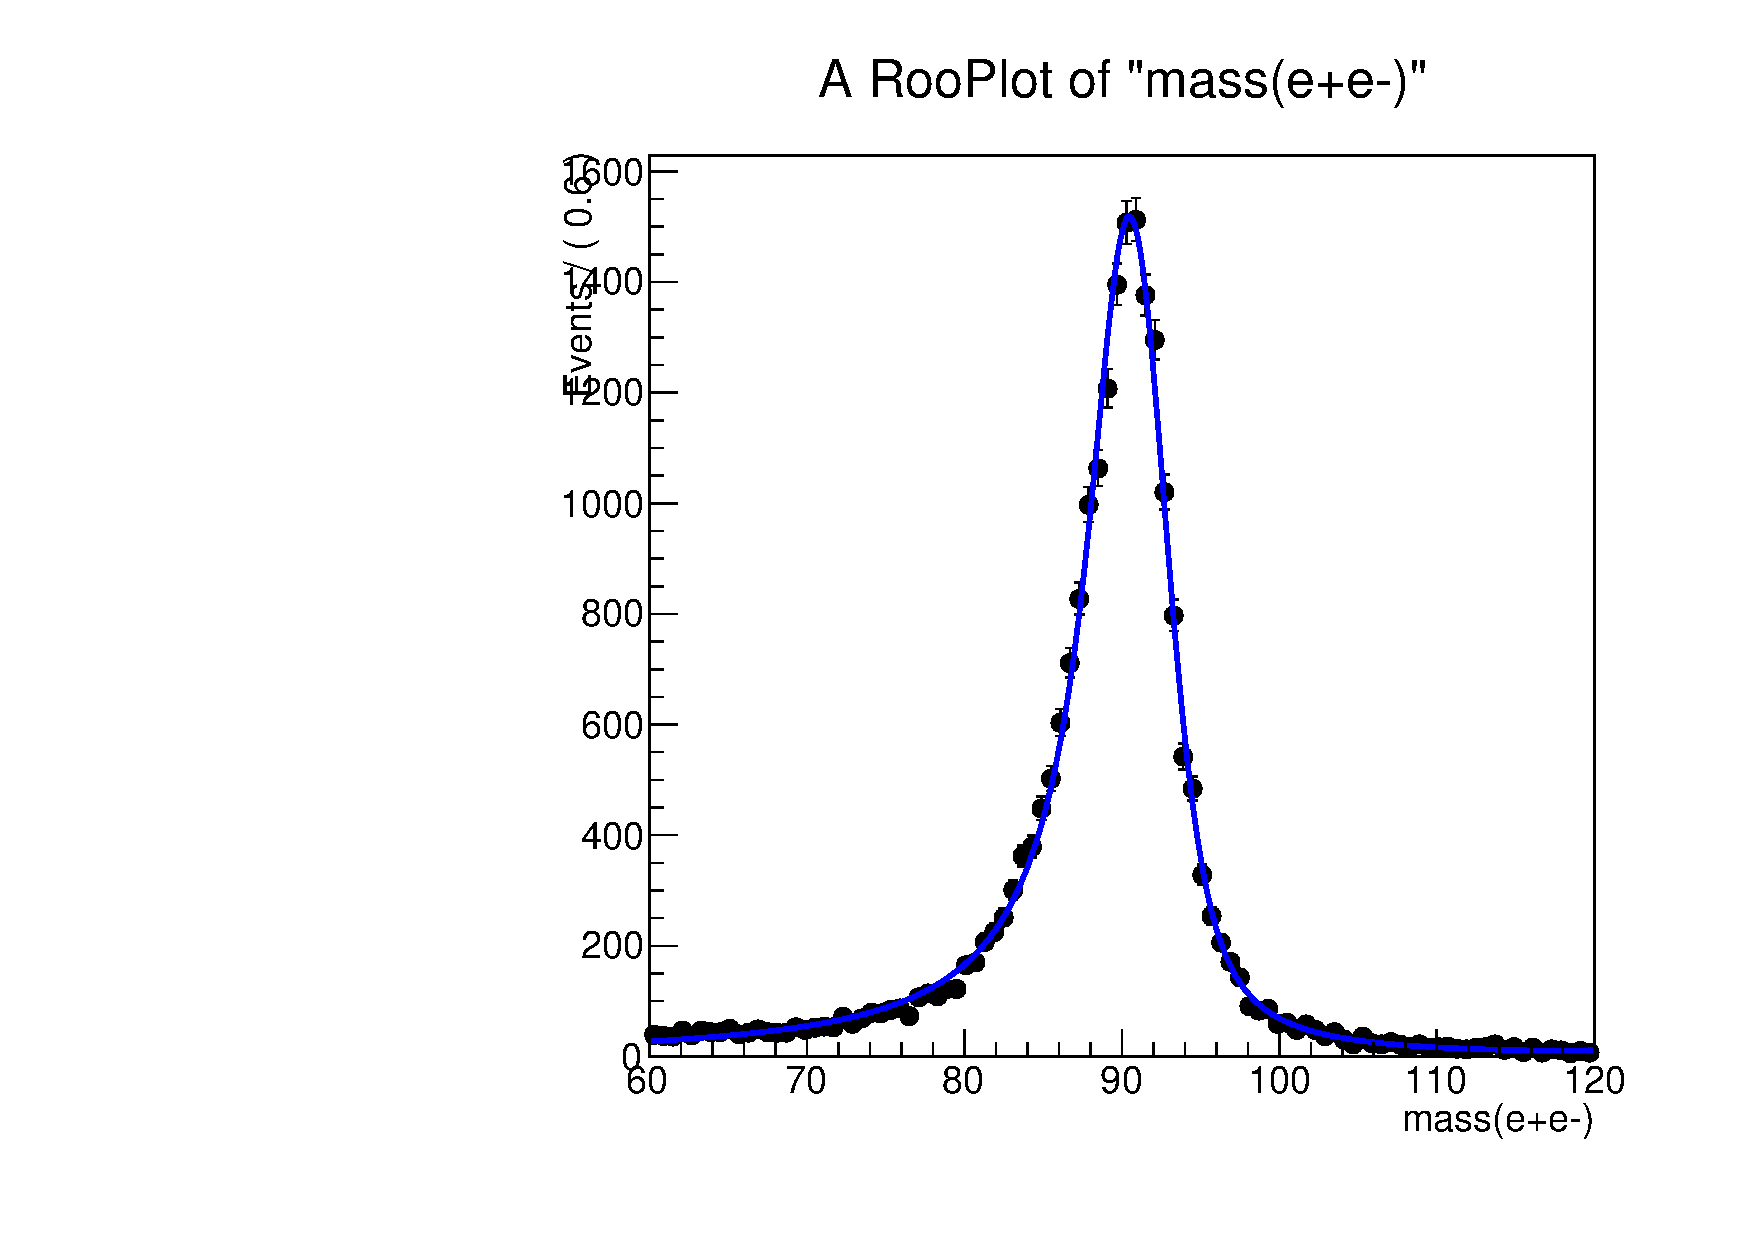
\includegraphics[width=2.0in]{Zee_conv.pdf}
    \caption{Invariant mass spectrum fit with a Relativistic Breit-Wigner distribution convoluted with a Crystal Ball distribution.}
    \label{fig:Zee_conv}
\end{figure} 

This code is intended to fit the mass spectrum with a Relativistic
Breit-Wigner distribution convoluted with a Crystal Ball distribution,
which you can read more about on
\href{http://en.wikipedia.org/wiki/Crystal_Ball_function}{Wikipedia}. The
Crystal Ball distribution is essentially a Gaussian distirbution with
a longer tail on one side,
\begin{equation}
f(x) = \left \{ \begin{array}{c}
 (\frac{n}{|\alpha|})^ne^{-\alpha^2/2} (\frac{n}{|\alpha|}-|\alpha|-x)^{-n}, x <-|\alpha|\\
 e^{-(x-\mu)^2/2\sigma^2}, x\geq-|\alpha|
\end{array} \right .
\end{equation}

Notice the fit is even better with respect to the last iteration. Why
is this so? Why did this homework (especially the final section with
the convolution) require the installation of a fast fourier transform (FFT) library?


\section{Further Discussion and Analysis}
The endpoint of an analysis is usually not performing a maximum
likelihood fit, but instead interpretting the output: the best-fit
parameter values (sometimes called the maximum likelihood estimators) and their uncertainties. 

\subsection{Retreiving the ML fit result}
From the text output of the code, you are given a series of numbers
representing the best-fit values and uncertainties for each
paramter. To complete the exercise you will need to find the best-fit
values for $\Gamma_Z$, the total width of the $Z$ boson, and $m_Z$,
the mass of the $Z$ boson. In the following, the best fit values for
these have been removed (so you can find and use your own numbers).
\clearpage
\begin{verbatim}
  RooFitResult: minimized FCN value: 71901, estimated distance to minimum: 7.7855e-07
                covariance matrix quality: Full, accurate covariance matrix
                Status : MIGRAD=0 HESSE=0 

    Floating Parameter  InitialValue    FinalValue +/-  Error     GblCorr.
  --------------------  ------------  --------------------------  --------
              GammaZee    2.4952e+00               +/-            <none>
                cbBias   -5.0000e-01    1.6158e+00 +/-  5.68e-01  <none>
                 cbCut    1.0500e+00    1.1297e+00 +/-  6.51e-02  <none>
               cbPower    2.4500e+00    1.6536e+00 +/-  1.04e-01  <none>
               cbSigma    5.7000e+00    1.6482e+00 +/-  8.28e-02  <none>
                    mZ    9.1188e+01               +/-             <none>
\end{verbatim}

\subsection{Determining the Number of Light Neutrinos}
The standard model, whose particle content is depicted in
Fig.~\ref{fig:sm}, contains three families of light neutrinos:
$\nu_e$, $\nu_{\mu}$, and $\nu_{\tau}$. 
\begin{figure}
    \centering
    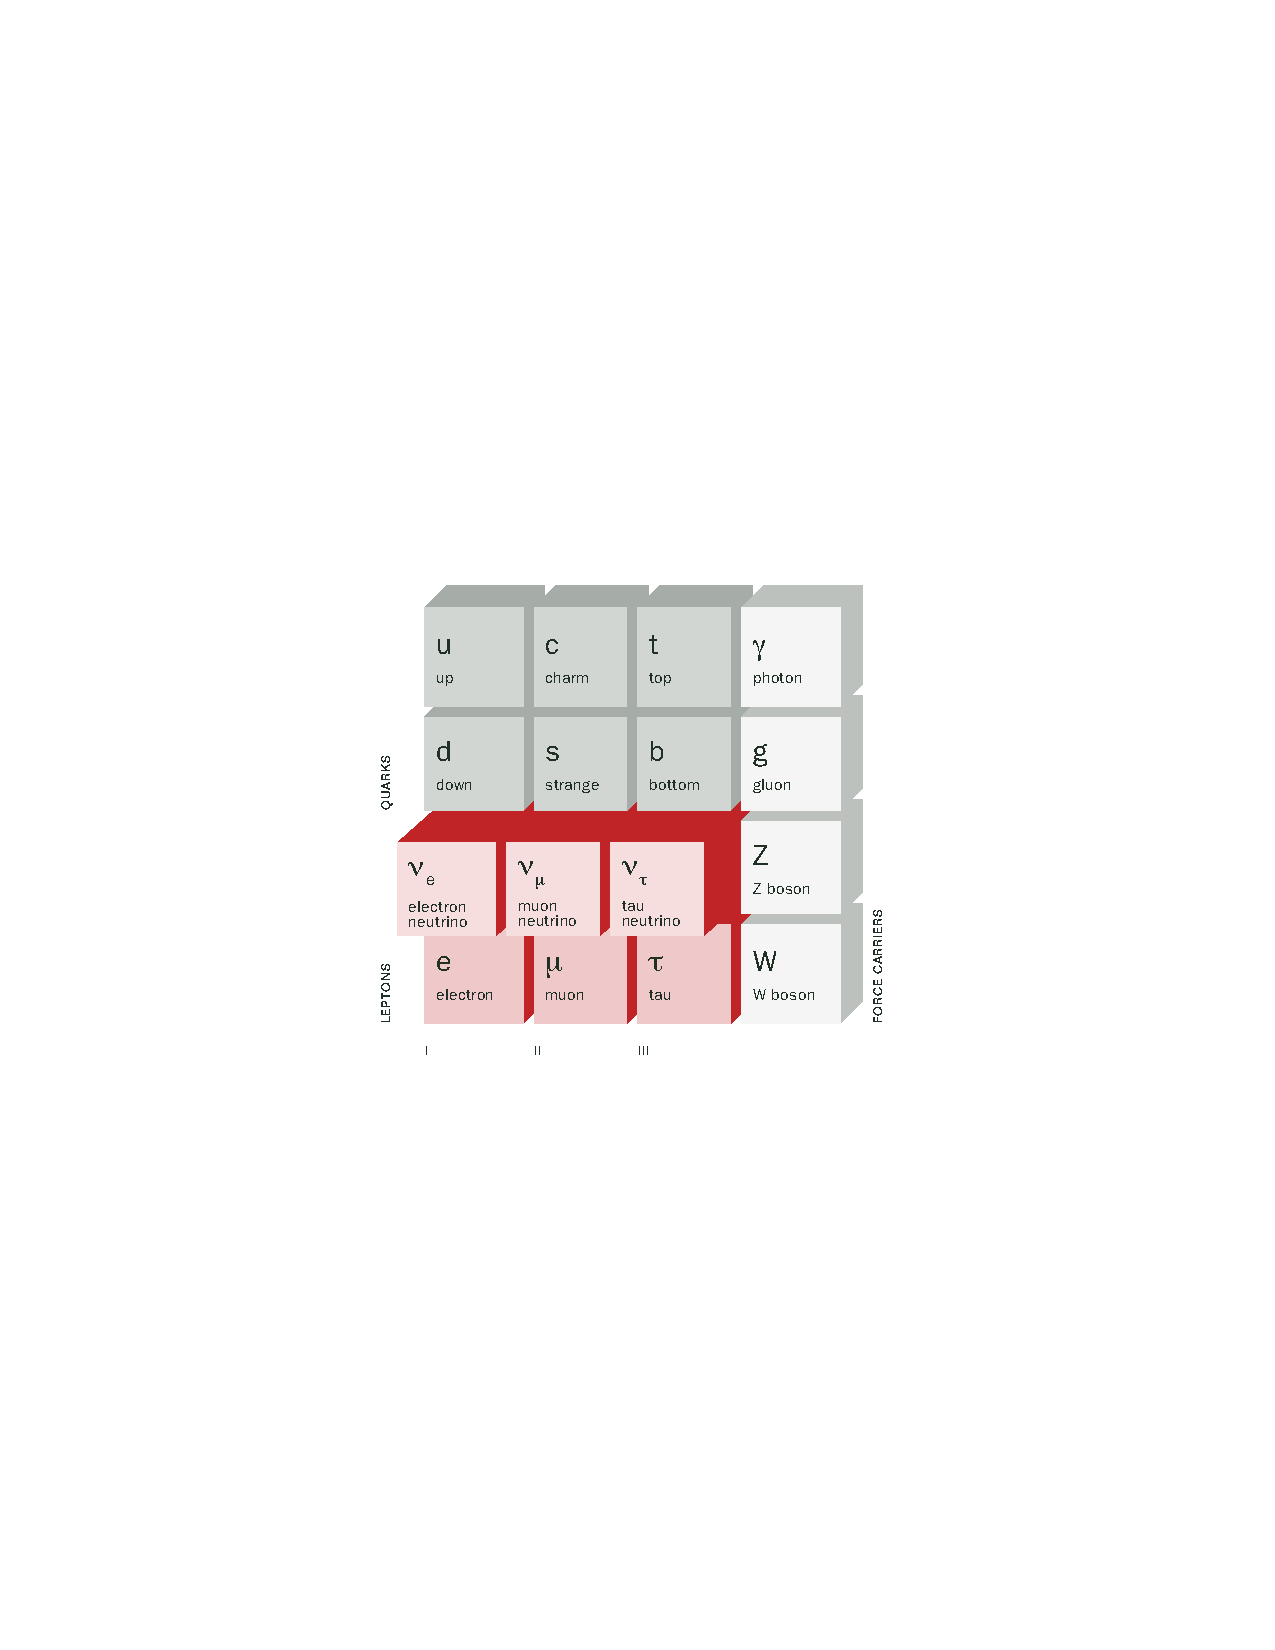
\includegraphics[width=3.0in,clip=true,viewport=150 250 500 550]{neutrino_pamphlet8.pdf}
    \caption{Particles in the standard model of particle physics.}
    \label{fig:sm}
\end{figure} 
The $Z$ boson has many observable decay modes including 
\begin{itemize}
\item $Z\to e^+e^-$
\item $Z\to \mu^+\mu^-$
\item $Z\to \tau^+\tau^-$
\item $Z\to u\bar{u}$
\item $Z\to d\bar{d}$
\item $Z\to c\bar{c}$
\item $Z\to s\bar{s}$
\item $Z\to b\bar{b}$
\end{itemize}
The $Z$ boson also has several \emph{invisible} decay modes. In the standard
model, the invisible decay modes are
\begin{itemize}
\item $Z\to \nu_e\bar\nu_e$
\item $Z\to \nu_{\mu}\bar\nu_{\mu}$
\item $Z\to \nu_{\tau}\bar\nu_{\tau}$
\end{itemize}
one for each flavor of neutrino.

\emph{Section under construction...}

\end{document}